% dernière modif : Alex 08/09 10h20

\documentclass[11pt]{article}

\usepackage[utf8]{inputenc}
\usepackage[table]{xcolor}
\usepackage[T1]{fontenc}
\usepackage[french]{babel}
\usepackage{natbib}
\usepackage[normalem]{ulem}
\usepackage{verbatim}
\usepackage{xcolor}
\usepackage{graphicx}
\usepackage{graphics}
\usepackage{fancybox}
\usepackage{amsfonts}
\usepackage{xcolor}
\usepackage{amsmath}
\usepackage{ulem}
\usepackage{adjustbox}
\usepackage{amssymb,amsmath,latexsym}
\usepackage{mathrsfs}
\usepackage[a4paper]{geometry}
\usepackage{subfig}
\usepackage[bottom]{footmisc}
\usepackage{default}
\usepackage{placeins}
\usepackage{float}
\usepackage{hyperref}
\usepackage{url}
%\usepackage{minted}

%\PassOptionsToPackage{hyphens}{url}\usepackage{hyperref}

%TITRE
\geometry{hscale=0.85,vscale=0.85,centering}
\title{Fiche Projet SOSI\\\huge{Brouilleur d'écran}}
\author{\emph{Superviseur} : Nicolas \textsc{Malandain} ~\\\\ \emph{Auteurs} : Gautier \textsc{Darchen}, Enora \textsc{Gicquel}, Alexandre \textsc{Huat}, Romain \textsc{Judic}}
\date{\today}

\begin{document}
\maketitle
\noindent\rule{\textwidth}{1.3pt}

Cette fiche résume le projet SOSI \emph{Brouilleur d'écran}. Nous rappellerons le sujet du projet puis présenterons notre travail.

\section{Rappel du sujet du projet}
Ce projet consiste à créer un programme qui brouille ou masque l'écran de l'ordinateur portable lorsque la webcam intégrée détecte un autre visage, l'objectif étant de protéger l'espace de travail de l'utilisateur.

\section{Travail réalisé}

\begin{figure}[H]
\begin{center}
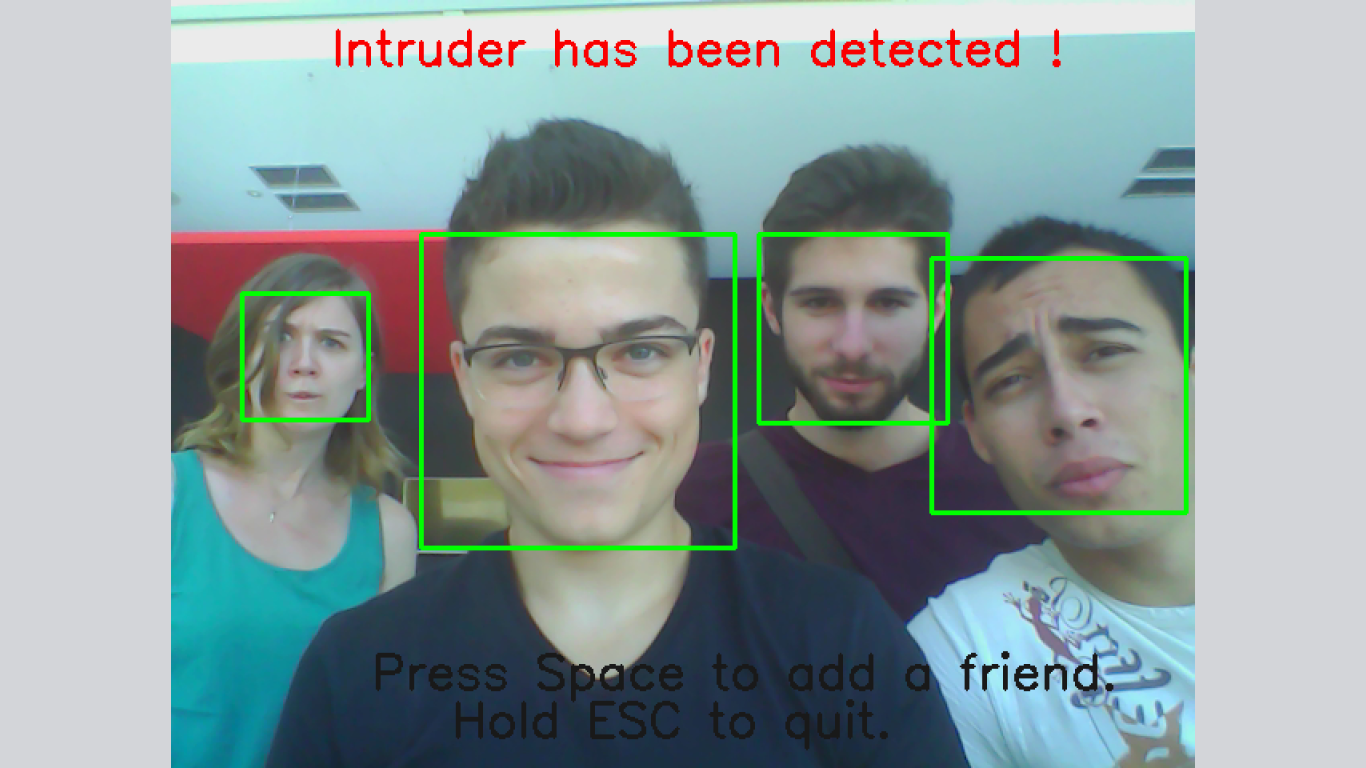
\includegraphics[width=0.4\textwidth]{capture.png}
\caption{Capture d'écran du brouilleur}
\end{center}
\end{figure}

\subsection{Ce que fait notre programme}
Notre programme empêche des tierces personnes de regarder l'écran de l'utilisateur à son insu. Lorsqu'un visage supplémentaire est détecté par la webcam, l'image filmée est affichée en plein écran de sorte à masquer l'intégralité de l'espace de travail. L'utilisateur peut alors :
\begin{itemize}
\item désactiver complètement le programme en maintenant la touche \texttt{ESC} ;
\item autoriser la nouvelle personne détectée à regarder l'écran en appuyant sur la barre d'espace ou lui demander de partir puis appuyer sur espace pour reprendre la main. L'espace de travail redevient visible mais le programme est toujours actif.
\end{itemize}

Quand une personne quitte le champ de vision, le nombre de visages autorisé est décrémenté. Le minimum de visages autorisé est 1. Les visages ne sont pas détectés à plus de 3 mètres (environ) et la détection ne marche que si le visage est à la verticale et de face.

Nous avons choisi d'afficher le film de la webcam plutôt que brouiller l'écran de l'ordinateur car c'est plus interactif et l'utilisateur peut directement savoir qui l'espionne. Les visages ne sont pas détectés en dessous de 3 mètres pour que l'utilisateur ne soit pas trop perturbé par un simple passant et parce qu'au delà, il est de toute façon dur de voir ou lire ce qu'il y a à l'écran.

\subsection{Notre choix technique}

Nous avons travaillé en Python avec OpenCV \cite{install_opencv}. OpenCV est une bibliothèque qui permet de faire du traitement d'image. Une recherche en ligne nous a permis de trouver un petit programme pour la reconnaissance faciale \cite{prog}. Un fichier XML \cite{xml} contient les données nécessaires pour la détection. OpenCV est aussi utilisable en C, C++, Java et d'autres langages. Nous avons choisi  d'utiliser Python car nous voulions découvrir ce langage.

\subsection{Organisation du travail}

Nous nous sommes divisés en deux groupes, l'un améliorant la détection des visages (Gautier et Romain), l'autre travaillant sur l'IHM (Enora et Alexandre). Nous n'avons pas rencontré de difficultés particulières.

\begin{description}
\item[Détection des visages :] Les fonctions de reconnaissance faciale proposées par OpenCV détectent beaucoup de faux positifs (visages dans des chemises, etc.). Ne pouvant modifier le fichier XML associé à ces fonctions, nous avons éliminé les parasites en ne considérant que les visages détectés sur plus de 100 images successives\footnote{Les faux positifs apparaissent sur peu d'images.}. 
\item[IHM :] L'IHM est très simple. Le film de la webcam est affiché en miroir et nous avons ajouté du texte sur l'image pour informer de la présence d'un intrus et dire à l'utilisateur ce qu'il peut faire.
\end{description}

\subsection{Utilisation du programme}
On lance le programme en exécutant la commande \texttt{python brouilleur\_SOSI.py}. Nous avons rajouté des modes \emph{glande} (\texttt{python brouilleur\_SOSI.py -glande}) où l'écran est masqué par un écran de travail (code Java) pour faire semblant de travailler, et \emph{Ironman} (\texttt{python brouilleur\_SOSI.py -iron}) où le visage d'Ironman recouvre les visages sur le film de la caméra\cite{opencv_moust}.

\subsection{Améliorations possibles}
\begin{itemize}
\item Permettre la détection d'un visage penché sur le côté ou à l'envers.
\item Activer le brouilleur uniquement quand une autre personne regarde l'écran \emph{(eye-tracker)}.
\item Reconnaître le visage précis de l'utilisateur pour n'autoriser que lui.
\end{itemize}

\bibliographystyle{alpha}
\bibliography{bib_sosi}



%%%% Commande pour lancer le programme
\end{document}